\documentclass[12pt, a4paper]{article}
\title{Дифракция света на ультразвуковой волне (4.3.2)}
\author{Стеценко Георгий, Б02-312}
\date{}
% !TeX encoding = UTF-8

\usepackage{geometry}
\usepackage{amsmath, amsfonts, amssymb, amsthm} % стандартный набор AMS-пакетов для математ. текстов
\usepackage{mathtext}
\usepackage[utf8]{inputenc} % кодировка utf8
\usepackage[russian]{babel} % русский язык
\usepackage[pdftex,dvipsnames]{xcolor} % работа с цветами
\usepackage[pdftex]{graphicx} % графика (картинки)
\usepackage{tikz,pgfplots} % рисунки
\usepackage{indentfirst}
%\usepackage[labelfont=bf,labelsep=endash,skip=3pt]{caption} % подпись картинок
% \usepackage{fancyhdr,pageslts} % настройка колонтитулов
\usepackage{enumitem} % работа со списками
\usepackage{floatrow,multicol,multirow,longtable,hhline} % работа с таблицами
\usepackage{float,wrapfig} % плавающие объекты
\usepackage{tcolorbox} % рамка вокруг текста
%\usepackage[calc]{datetime2} % дата
\usepackage{bm} % жирное начертание в формулах
\usepackage{physics} % физический пакет
\DeclareMathAlphabet\mathbfcal{OMS}{cmsy}{b}{n}
\usepackage{pgfornament} % красивые рюшечки и вензеля
\usepackage{mdframed}
\usepackage{derivative}
\usepackage{mathrsfs} %EDS
\usepackage{soul} % strikethorugh
%\usepackage{boondox-cal}

% ----------------------------------------
% Настройка шрифта

% Просто закооментируйте следующую строчку, если не работает. Будет другой шрифт, правда :(
% \usepackage{pscyr}

% ----------------------------------------
% Стилевые настройки

\usepackage{boldline} % жирная линия после таблиц (чтобы не было ошибок, этот пакет должен подключаться именно тут!)
\floatsetup[table]{style=Plaintop,floatrowsep=qquad} % настройка оформления таблиц
\setlist[enumerate,itemize]{leftmargin=5mm,itemindent=10mm,itemsep=0mm,
listparindent=0em,labelsep=2mm,topsep=2mm,labelwidth=4mm} % настройки списков

\setlength{\columnsep}{0.5cm} % расстояние между колонками
\setlength{\parskip}{1pt} % расстояние до текста от колонтитула

%\usepackage{titlesec} % управление оформлением section
%\renewcommand{\thesection}{\Roman{section}}
%\titleformat{\section}[block]{\bfseries\large}{\thesection.}{5pt}{}

% ----------------------------------------
% Настройки полей
\geometry{
  left=10mm,
  top=10mm,
  right=10mm,
  bottom=15mm,
  marginparsep=0mm,
  marginparwidth=0mm,
  headheight=0pt,
  headsep=0pt,
footskip=20pt}

% ----------------------------------------
% Настройки колонтитулов и нумерации страниц
\pagenumbering{arabic}



\newcounter{ntask}
\setcounter{ntask}{0}


\newcommand{\arsh}{\mathrm{arsh} \,\,}
\newcommand{\arch}{\mathrm{arch} \,\,}
\newcommand{\arth}{\mathrm{arth} \,\,}
\newcommand{\arcth}{\mathrm{arcth} \,\,}
\renewcommand{\Re}{\operatorname{Re} \,}
\newcommand{\EDS}{\mathscr{E}}
\newcommand{\diffract}[1]{\frac{\mathrm{d}#1}{\mathrm{d}t}}

\newcommand{\kHz}{~\mathrm{kHz}}
\newcommand{\GHz}{~\mathrm{GHZ}}
\newcommand{\us}{~\mathrm{\mu s}}
\addto\captionsrussian{\def\refname{Источники}}

\begin{document}
\maketitle

\section{Аннотация}
\textbf{Цель работы:} Изучение дифракции света на синусоидальной акустической 
решётке и наблюдение фазовой решётки методом тёмного поля.

\textbf{Оборудование и материалы:} оптическая скамья, осветитель, два длиннофокусных 
объектива, кювета с жидкостью, кварцевый излучатель с микрометрическим винтом, 
генератор ультразвуковой частоты, линза, вертикальная нить на рейтере, микроскоп.

\section{Теоретические сведения}
При прохождении ультразвуковой волны через жидкость в ней возникают периодические неоднородности
коэффициента преломления, создаётся фазовая решётка, которую мы считаем неподвижной ввиду
малости скорости звука относительно скорости света. Показатель преломления $n$ изменяется
по закону:

\begin{equation}
  n = n_0 (1 + m \cdot \cos \Omega x)
\end{equation}
Здесь $\Omega = 2\pi / \Lambda$ -- волновое число для ультразвуковой волны, $m \ll 1$ -- глубина 
модуляции $n$.

Положим фазу $\varphi$ колебаний на передней стенке кюветы равной нулю, тогда на задней 
поверхности она равна:
\begin{equation}
  \varphi = knL = \varphi_0 (1 + m\cdot \cos \Omega x)
\end{equation}
где $k = 2\pi / \lambda$ -- волновое число света, $L$ -- длина кюветы, $\varphi_0 = kn_0 L$ -- константа. 

Тогда кювету можно считать чисто фазовой решёткой с фазовым пропусканием  
$$t(x) = \exp (im \cos (\Omega x))$$
Полагая, что глубина модуляции $m \ll 1$, получим $t(x) \approx 1 + im \cos \Omega x = 1 + im/2 \left( e^{i\Omega x} + e^{-i\Omega x}\right)$.
При освещении этой решётки плоской нормально падающей волной амплитуды $a$ имеем за решёткой:
$$f(x,z) = a \exp (ikz) + \frac{iam}{2} \exp i(\Omega x + \sqrt{k^2 - \Omega^2}z) + \frac{iam}{2} \exp i(-\Omega x + \sqrt{k^2 - \Omega^2}z)$$

По сути в случае идеальной фазовой решётки имеем три дифракционных максимума Фраунгофера, собираемых линзой 
в своей фокальной плоскости. 

\section{Экспериментальная установка}
Источник света Л через светофильтр Ф и конденсор К освещает щель S, 
которая расположена в фокусе объектива $О_1$. Выходящий из объектива
параллельный пучок света проходит через кювету $C$ перпендикулярно 
направлению распространения УЗ-волн. Эти волны возбуждаются в жидкости 
пьезокварцевой пластинкой $Q$, прикреплённой к стенке кюветы. На 
кварцевую пластинку подаётся напряжение ультразвуковой частоты от
генератора (на рисунке не показан). В фокальной плоскости второго 
объектива $О_2$ образуется дифракционная картина, наблюдаемая при 
помощи микроскопа $М$. При этом обязательно применяют 
монохроматическое излучение (красный светофильтр).

\begin{figure}[h]
  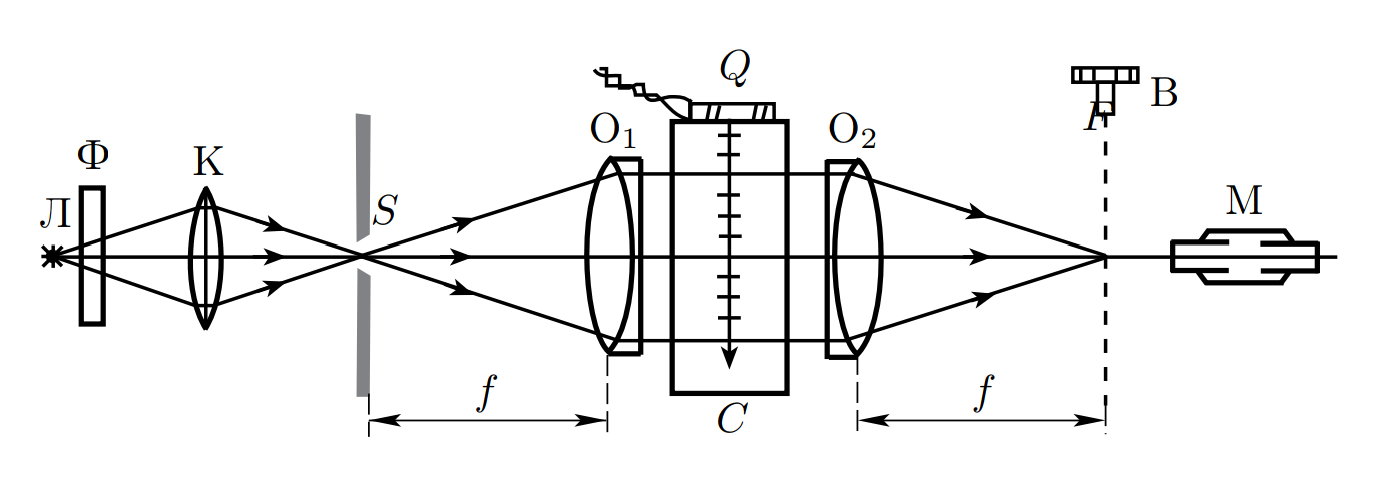
\includegraphics[width=0.8\linewidth]{pics/setup.png}
  \caption{Схема установки}
\end{figure}

\begin{figure}[H]
  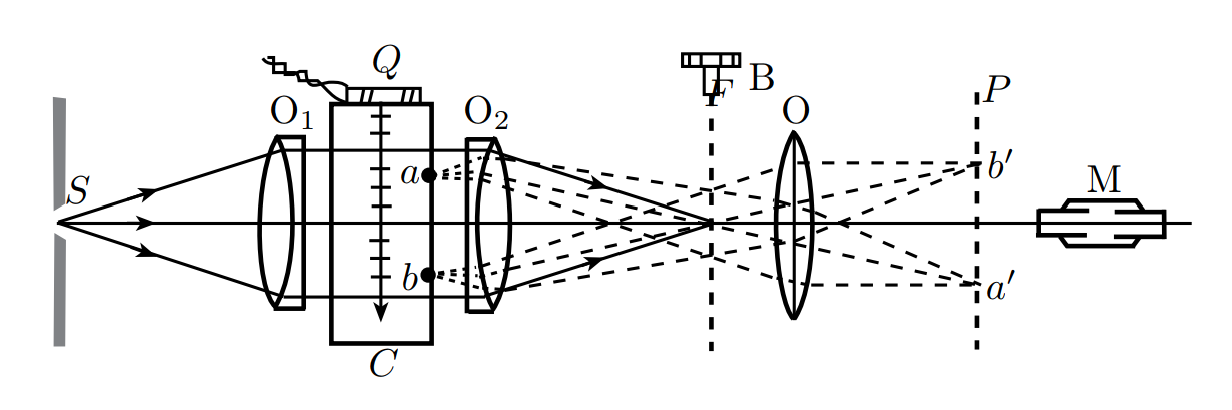
\includegraphics[width=0.8\linewidth]{pics/setup-2.png}
  \caption{Схема установки для измерения методом тёмного поля}
\end{figure}
Теперь получим изображение фазовой решётки. Для этого используем метод <<тёмного поля>> -- 
закрывания центрального максимума в дифракционной картине с помощью тонкой нити и на рейтере. 
В поле зрения микроскопа при этом образуется изображение фазовой решётки с шириной линии
$\Lambda/2$, где $\Lambda$ -- длина УЗ-волны в воде.

Данные об установке:
\begin{itemize}
  \item \textbf{Фокусное расстояние линзы O2 }$F_2 = 28~\mathrm{cm}$;
  \item \textbf{Длина волны }$\lambda = (640\pm20)~\mathrm{nm}$.
\end{itemize}

\section{Методика измерений и результаты}
\subsection{Определение скорости ультразвука по дифракционной картине}
Для начала получим дифракционную картину. Отчётливо видны отдельные полосы, при этом при увеличении
мощности генератора полос становится заметно больше (вплоть до 11).

Снимем зависимость отсчётов микрометрического винта в зависимости от номера полосы, а также частоты
генератора:
\begin{table}[H]
  \centering
  \begin{tabular}{|c|c|}
      \hline
      Частота ($\text{МГц}$) & Отсчёты \\ \hline
      1.07188 & 11, 53, 86, 125, 164, 203, 240 \\ \hline
      1.19215 & 69, 113, 155, 191, 233, 279, 326, 365, 409 \\ \hline
      1.24837 & 0, 39, 76, 119, 164 \\ \hline
      2.89424 & 36, 141, 244, 345, 449, 554, 656 \\ \hline
      4.83451 & 75, 248, 418 \\ \hline
  \end{tabular}
  \caption{Зависимость счетчиков от частоты.}
  \label{freq_counts_table}
\end{table}
Принимаем во внимание, что один отсчёт винта соответсвует $4~\mathrm{\mu m}$.
Найдём тогда линеаризацией соответсвующие ширины дифракционных полос:
\begin{figure}[H]
  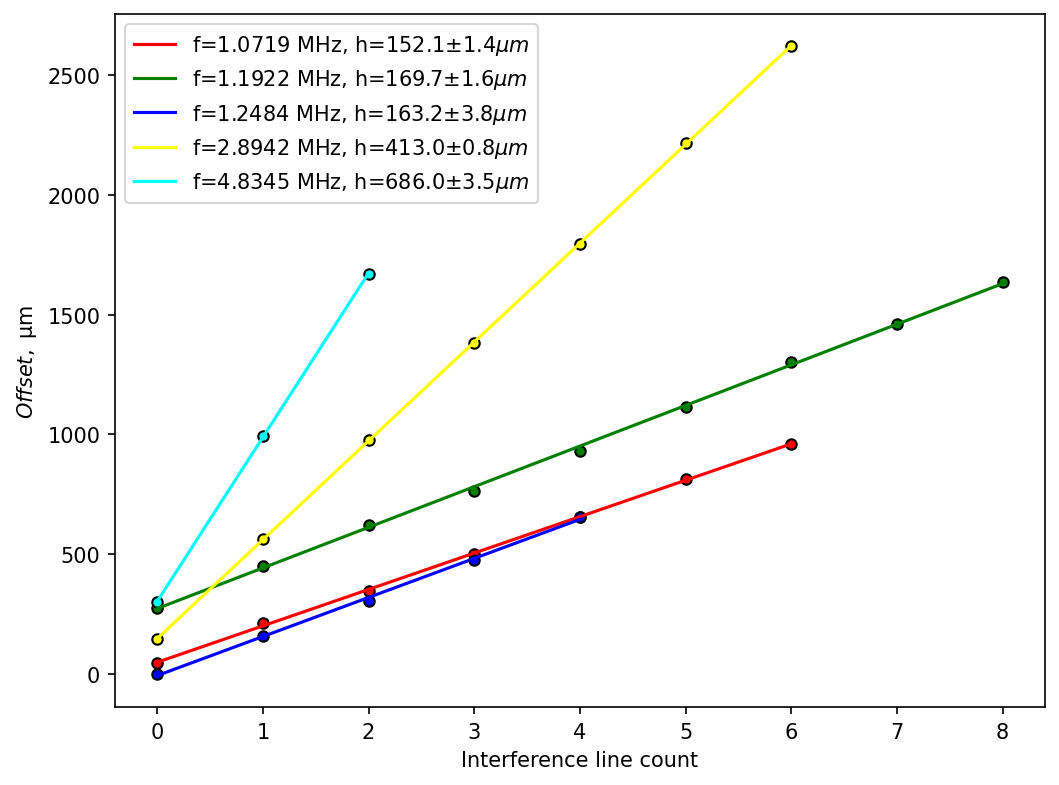
\includegraphics[width=0.75\linewidth]{pics/line count.png}
\end{figure}
Тогда справедливо следующее:
$$\Lambda = v/f, \quad h(f) \approx F_2 \cdot \theta(f) = F_2 \cdot \lambda/\Lambda = \lambda F_2 f / v \quad(\theta \ll 1)$$
$$h = \frac{\lambda F_2}{v} f$$
Согласно данной зависимости линеаризуем:
\begin{figure}[H]
  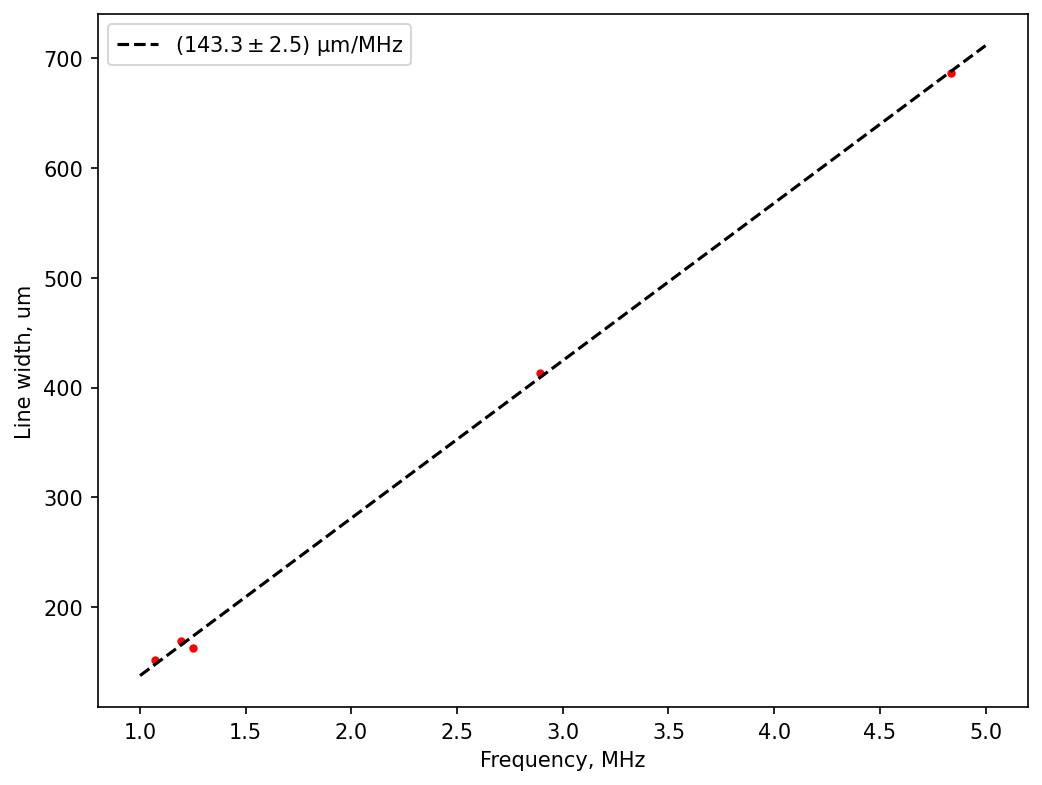
\includegraphics[width=0.75\linewidth]{pics/speed_of_sound_1.png}
\end{figure}
И получаем значение $v = \lambda F_2 / k = (1250\pm60)~\mathrm{m/s}$,
что вообще-то достаточно далеко от табличного значения в $1490~\mathrm{m/s}$...

\subsection{Измерение методом тёмного поля}
При нормировке собственной шкалы микроскопа по линейке, на которую он сфокусирован, оказалось, что
1 мм линейки соответсвует ($15.5\pm0.5$)делениям шкалы.

Ввиду количества данных, они сразу приведены в графическом виде для удобства.
\begin{figure}[H]
  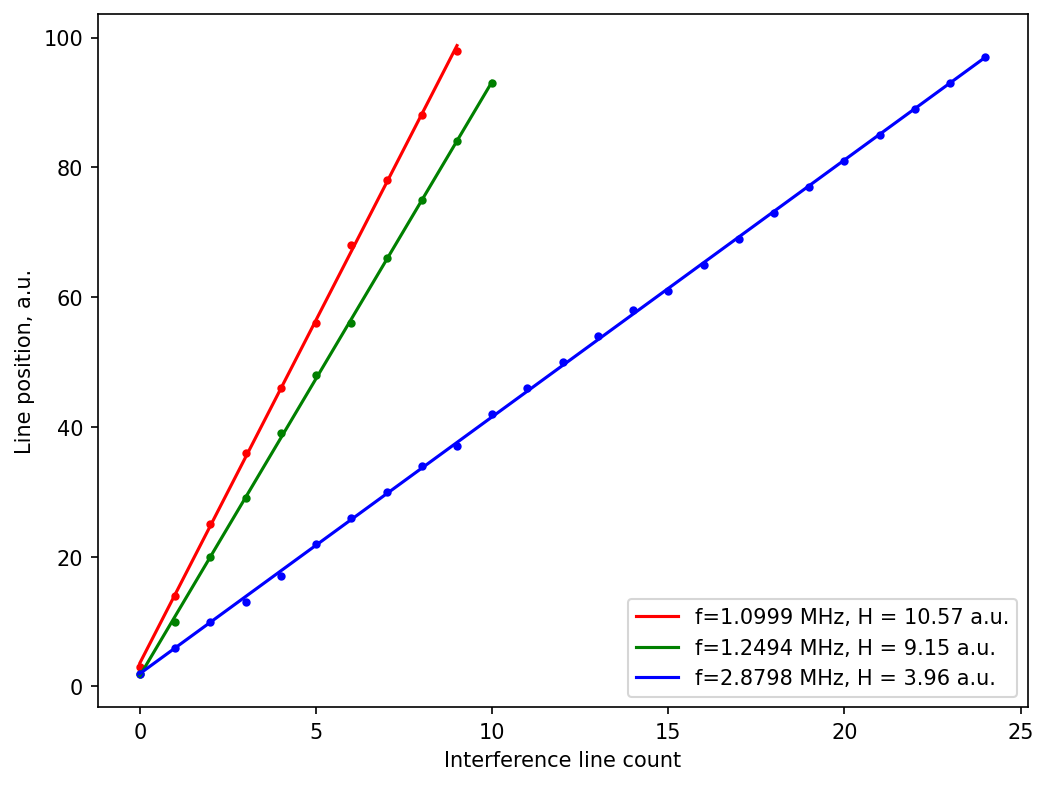
\includegraphics[width=0.75\linewidth]{pics/dark field.png}
\end{figure}

По полученным данным рассчитаем соотвествующие скорости звука в воде:
\begin{table}[H]
  \begin{tabular}{|l|l|l|l|}
  \hline
  f, MHz & H, a.u. & $H_\text{toscale}$, mm & $v$, m/s \\ \hline
  1.0999 & 10.57   & 0.705          & 1500   \\ \hline
  1.2494 & 9.15    & 0.610          & 1474   \\ \hline
  2.8798 & 3.96    & 0.264          & 1470   \\ \hline
  \end{tabular}
\end{table}

Таким образом, этим методом получено $v = (1480\pm50)~\mathrm{m/s}$, что уже гораздо лучше совпадает с табличным значением.
\section{Обсуждение результатов и выводы}
В данной работе были получены дифракционные картины на стоячей волне сжатия в воде, а так же
изображение фазовой решётки методом тёмного поля. Были получены оценки скорости ультразвуковых волн
в воде, при этом первая подозрительно отличается от табличного значения в 1.25 раз... Есть подозрение,
что шаг микрометрического винта составлял $5\mathrm{mu m}$ вместо $4\mathrm{mu m}$ -- в таком случае оба значения
скорости ультразвука сошлись бы с табличным.
\end{document}
